\documentclass[journal,12pt,twocolumn]{IEEEtran}
%
\usepackage{setspace}
\usepackage{gensymb}
%\doublespacing
\singlespacing

%\usepackage{graphicx}
%\usepackage{amssymb}
%\usepackage{relsize}
\usepackage[cmex10]{amsmath}
%\usepackage{amsthm}
%\interdisplaylinepenalty=2500
%\savesymbol{iint}
%\usepackage{txfonts}
%\restoresymbol{TXF}{iint}
%\usepackage{wasysym}
\usepackage{amsthm}
%\usepackage{iithtlc}
\usepackage{mathrsfs}
\usepackage{txfonts}
\usepackage{stfloats}
\usepackage{bm}
\usepackage{cite}
\usepackage{cases}
\usepackage{subfig}
%\usepackage{xtab}
\usepackage{longtable}
\usepackage{multirow}
%\usepackage{algorithm}
%\usepackage{algpseudocode}
\usepackage{enumitem}
\usepackage{mathtools}
\usepackage{tikz}
\usepackage[american]{circuitikz}
\usepackage{verbatim}
\usepackage{tfrupee}
\usepackage[breaklinks=true]{hyperref}
%\usepackage{stmaryrd}
\usepackage{tkz-euclide} % loads  TikZ and tkz-base
\usetkzobj{all}
\usetikzlibrary{decorations.markings}
\usetikzlibrary{shapes.geometric}
\newif\iflabrev
\usepackage{listings}
    \usepackage{color}                                            %%
    \usepackage{array}                                            %%
    \usepackage{longtable}                                        %%
    \usepackage{calc}                                             %%
    \usepackage{multirow}                                         %%
    \usepackage{hhline}                                           %%
    \usepackage{ifthen}                                           %%
  %optionally (for landscape tables embedded in another document): %%
    \usepackage{lscape}     
\usepackage{multicol}
\usepackage{chngcntr}
%\usepackage{enumerate}

%\usepackage{wasysym}
%\newcounter{MYtempeqncnt}
\DeclareMathOperator*{\Res}{Res}
%\renewcommand{\baselinestretch}{2}
\renewcommand\thesection{\arabic{section}}
\renewcommand\thesubsection{\thesection.\arabic{subsection}}
\renewcommand\thesubsubsection{\thesubsection.\arabic{subsubsection}}

\renewcommand\thesectiondis{\arabic{section}}
\renewcommand\thesubsectiondis{\thesectiondis.\arabic{subsection}}
\renewcommand\thesubsubsectiondis{\thesubsectiondis.\arabic{subsubsection}}

% correct bad hyphenation here
\hyphenation{op-tical net-works semi-conduc-tor}
\def\inputGnumericTable{}                                 %%

\lstset{
%language=C,
frame=single, 
breaklines=true,
columns=fullflexible
}
%\lstset{
%language=tex,
%frame=single, 
%breaklines=true
%}

\begin{document}
%


\newtheorem{theorem}{Theorem}[section]
\newtheorem{problem}{Problem}
\newtheorem{proposition}{Proposition}[section]
\newtheorem{lemma}{Lemma}[section]
\newtheorem{corollary}[theorem]{Corollary}
\newtheorem{example}{Example}[section]
\newtheorem{definition}[problem]{Definition}
%\newtheorem{thm}{Theorem}[section] 
%\newtheorem{defn}[thm]{Definition}
%\newtheorem{algorithm}{Algorithm}[section]
%\newtheorem{cor}{Corollary}
\newcommand{\BEQA}{\begin{eqnarray}}
\newcommand{\EEQA}{\end{eqnarray}}
\newcommand{\define}{\stackrel{\triangle}{=}}
\bibliographystyle{IEEEtran}
%\bibliographystyle{ieeetr}
\providecommand{\mbf}{\mathbf}
\providecommand{\pr}[1]{\ensuremath{\Pr\left(#1\right)}}
\providecommand{\qfunc}[1]{\ensuremath{Q\left(#1\right)}}
\providecommand{\sbrak}[1]{\ensuremath{{}\left[#1\right]}}
\providecommand{\lsbrak}[1]{\ensuremath{{}\left[#1\right.}}
\providecommand{\rsbrak}[1]{\ensuremath{{}\left.#1\right]}}
\providecommand{\brak}[1]{\ensuremath{\left(#1\right)}}
\providecommand{\lbrak}[1]{\ensuremath{\left(#1\right.}}
\providecommand{\rbrak}[1]{\ensuremath{\left.#1\right)}}
\providecommand{\cbrak}[1]{\ensuremath{\left\{#1\right\}}}
\providecommand{\lcbrak}[1]{\ensuremath{\left\{#1\right.}}
\providecommand{\rcbrak}[1]{\ensuremath{\left.#1\right\}}}
\theoremstyle{remark}
\newtheorem{rem}{Remark}
\newcommand{\sgn}{\mathop{\mathrm{sgn}}}
\providecommand{\abs}[1]{\left\vert#1\right\vert}
\providecommand{\res}[1]{\Res\displaylimits_{#1}} 
\providecommand{\norm}[1]{\left\lVert#1\right\rVert}
%\providecommand{\norm}[1]{\lVert#1\rVert}
\providecommand{\mtx}[1]{\mathbf{#1}}
\providecommand{\mean}[1]{E\left[ #1 \right]}
\providecommand{\fourier}{\overset{\mathcal{F}}{ \rightleftharpoons}}
%\providecommand{\hilbert}{\overset{\mathcal{H}}{ \rightleftharpoons}}
\providecommand{\system}{\overset{\mathcal{H}}{ \longleftrightarrow}}
	%\newcommand{\solution}[2]{\textbf{Solution:}{#1}}
\newcommand{\solution}{\noindent \textbf{Solution: }}
\newcommand{\cosec}{\,\text{cosec}\,}
\providecommand{\dec}[2]{\ensuremath{\overset{#1}{\underset{#2}{\gtrless}}}}
\newcommand{\myvec}[1]{\ensuremath{\begin{pmatrix}#1\end{pmatrix}}}
\newcommand{\mydet}[1]{\ensuremath{\begin{vmatrix}#1\end{vmatrix}}}
%\numberwithin{equation}{section}
\numberwithin{equation}{subsection}
%\numberwithin{problem}{section}
%\numberwithin{definition}{section}
\makeatletter
\@addtoreset{figure}{problem}
\makeatother
\let\StandardTheFigure\thefigure
\let\vec\mathbf
%\renewcommand{\thefigure}{\theproblem.\arabic{figure}}
\renewcommand{\thefigure}{\theproblem}
%\setlist[enumerate,1]{before=\renewcommand\theequation{\theenumi.\arabic{equation}}
%\counterwithin{equation}{enumi}
%\renewcommand{\theequation}{\arabic{subsection}.\arabic{equation}}
\def\putbox#1#2#3{\makebox[0in][l]{\makebox[#1][l]{}\raisebox{\baselineskip}[0in][0in]{\raisebox{#2}[0in][0in]{#3}}}}
     \def\rightbox#1{\makebox[0in][r]{#1}}
     \def\centbox#1{\makebox[0in]{#1}}
     \def\topbox#1{\raisebox{-\baselineskip}[0in][0in]{#1}}
     \def\midbox#1{\raisebox{-0.5\baselineskip}[0in][0in]{#1}}
\vspace{3cm}
\title{
%	\logo{
Control Systems
%	}
}
\author{ G V V Sharma$^{*}$% <-this % stops a space
	\thanks{*The author is with the Department
		of Electrical Engineering, Indian Institute of Technology, Hyderabad
		502285 India e-mail:  gadepall@iith.ac.in. All content in this manual is released under GNU GPL.  Free and open source.}
	
}	
%\title{
%	\logo{Matrix Analysis through Octave}{\begin{center}\includegraphics[scale=.24]{tlc}\end{center}}{}{HAMDSP}
%}
% paper title
% can use linebreaks \\ within to get better formatting as desired
%\title{Matrix Analysis through Octave}
%
%
% author names and IEEE memberships
% note positions of commas and nonbreaking spaces ( ~ ) LaTeX will not break
% a structure at a ~ so this keeps an author's name from being broken across
% two lines.
% use \thanks{} to gain access to the first footnote area
% a separate \thanks must be used for each paragraph as LaTeX2e's \thanks
% was not built to handle multiple paragraphs
%
%\author{<-this % stops a space
%\thanks{}}
%}
% note the % following the last \IEEEmembership and also \thanks - 
% these prevent an unwanted space from occurring between the last author name
% and the end of the author line. i.e., if you had this:
% 
% \author{....lastname \thanks{...} \thanks{...} }
%                     ^------------^------------^----Do not want these spaces!
%
% a space would be appended to the last name and could cause every name on that
% line to be shifted left slightly. This is one of those "LaTeX things". For
% instance, "\textbf{A} \textbf{B}" will typeset as "A B" not "AB". To get
% "AB" then you have to do: "\textbf{A}\textbf{B}"
% \thanks is no different in this regard, so shield the last } of each \thanks
% that ends a line with a % and do not let a space in before the next \thanks.
% Spaces after \IEEEmembership other than the last one are OK (and needed) as
% you are supposed to have spaces between the names. For what it is worth,
% this is a minor point as most people would not even notice if the said evil
% space somehow managed to creep in.
% The paper headers
%\markboth{Journal of \LaTeX\ Class Files,~Vol.~6, No.~1, January~2007}%
%{Shell \MakeLowercase{\textit{et al.}}: Bare Demo of IEEEtran.cls for Journals}
% The only time the second header will appear is for the odd numbered pages
% after the title page when using the twoside option.
% 
% *** Note that you probably will NOT want to include the author's ***
% *** name in the headers of peer review papers.                   ***
% You can use \ifCLASSOPTIONpeerreview for conditional compilation here if
% you desire.
% If you want to put a publisher's ID mark on the page you can do it like
% this:
%\IEEEpubid{0000--0000/00\$00.00~\copyright~2007 IEEE}
% Remember, if you use this you must call \IEEEpubidadjcol in the second
% column for its text to clear the IEEEpubid mark.
% make the title area
\maketitle
\newpage
\tableofcontents
\bigskip
\renewcommand{\thefigure}{\theenumi}
\renewcommand{\thetable}{\theenumi}
%\renewcommand{\theequation}{\theenumi}
%\begin{abstract}
%%\boldmath
%In this letter, an algorithm for evaluating the exact analytical bit error rate  (BER)  for the piecewise linear (PL) combiner for  multiple relays is presented. Previous results were available only for upto three relays. The algorithm is unique in the sense that  the actual mathematical expressions, that are prohibitively large, need not be explicitly obtained. The diversity gain due to multiple relays is shown through plots of the analytical BER, well supported by simulations. 
%
%\end{abstract}
% IEEEtran.cls defaults to using nonbold math in the Abstract.
% This preserves the distinction between vectors and scalars. However,
% if the journal you are submitting to favors bold math in the abstract,
% then you can use LaTeX's standard command \boldmath at the very start
% of the abstract to achieve this. Many IEEE journals frown on math
% in the abstract anyway.
% Note that keywords are not normally used for peerreview papers.
%\begin{IEEEkeywords}
%Cooperative diversity, decode and forward, piecewise linear
%\end{IEEEkeywords}
% For peer review papers, you can put extra information on the cover
% page as needed:
% \ifCLASSOPTIONpeerreview
% \begin{center} \bfseries EDICS Category: 3-BBND \end{center}
% \fi
%
% For peerreview papers, this IEEEtran command inserts a page break and
% creates the second title. It will be ignored for other modes.
%\IEEEpeerreviewmaketitle
\begin{abstract}
The objective of this manual is to introduce control system design at an elementary level.
\end{abstract}
\section{Feedback Circuits}
\begin{enumerate}[label=\thesubsection.\arabic*.,ref=\thesubsection.\theenumi]
\numberwithin{equation}{enumi}
\item
For the Wein-bridge oscillator of Fig \ref{fig:ee18btech11044_3_tikz_1}, use the expression for loop gain in Eq \ref{eq:ee18btech11044_3_1}  to find the poles of the closed-loop system. Give the expression for the pole , Q and use it to show that to locate the poles in the right half of s plane, $\frac{R_2}{R_1}$ must be selected to be greater than 2. 

\begin{figure}[!hbt]
	\begin{center}
			\resizebox{\columnwidth}{!}{\begin{circuitikz}
\ctikzset{bipoles/length=1cm}

\draw 
(0, 0) node[op amp] (opamp) {}
(opamp.-) -- (-1,0.35) -- (-1.5,0.35) to[R=$R_1$] (-3,0.35) -- (-3,0.33)node[ground]{}
(-1,0.35)-- (-1,1) to[R=$R_2$] (2,1) -- (2,0){}
(opamp.out)--(2,0){}
(opamp.+) -- (-1,-0.35) -- (-1,-1.5) to[C=$C$] (0.5,-1.5) to[R=$R$] (2,-1.5) -- (2,0){}
(-1,-1.5) -- (-1,-1.75)to[R=$R$] (-1,-2.5) -- (-1,-2.57)node[ground]{}
(0.5,-1.5) -- (0.5,-1.75) to[C=$C$] (0.5,-2.5) -- (0.5,-2.57)node[ground]{}
node at (2.3,0){$V_{out}$}



;\end{circuitikz}
}
	\end{center}
\caption{}
\label{fig:ee18btech11044_3_tikz_1}
\end{figure}


\item Compare the basic structure for a sinusoidal oscillator with Wein-bridge oscillator and give expressions for A and $\beta$. 

\solution
\begin{itemize}
    \item Comparring Fig \ref{fig:ee18btech11044_3_tikz_1} and Fig \ref{fig:ee18btech11044_3_tikz_2}, we get
\begin{align}
A = 1+\frac{R_2}{R_1} \\
\beta = \frac{Z_p}{Z_p + Z_s}
\end{align}
where,
\begin{align}
    Z_p = \frac{R}{RSC+1} \\
    Z_s = \frac{RSC+1}{SC}
\end{align}
\end{itemize}



\begin{figure}[!hbt]
	\begin{center}
		\resizebox{\columnwidth}{!}{\tikzstyle{block} = [draw, fill=white!20, rectangle, 
    minimum height=3em, minimum width=6em]
\tikzstyle{sum} = [draw, fill=white!20, circle, node distance=1cm]
\tikzstyle{input} = [coordinate]
\tikzstyle{output} = [coordinate]
\tikzstyle{pinstyle} = [pin edge={to-,thin,black}]

\begin{tikzpicture}[auto, node distance=2cm,>=latex']
    \node [input, name=input] {};
    \node [sum, right of=input] (sum) {};
    \node [block, right of=sum] (controller) {$Amplifier$};
    \node [output, right of=controller] (output) {};
    \node [block, below of=controller] (feedback) {\tiny{Frequency selective network}};
    
    \draw [->] (sum) -- node {$V_i$} (controller);
    \draw [->] (controller) -- node [name=y] {$V_o$}(output);
    \draw [->] (y) |- (feedback);
    \draw [->] (feedback) -| node[pos=0.99]{$+$}  node [near end] {$V_f$} (sum);
\end{tikzpicture}
}
	\end{center}
\caption{}
\label{fig:ee18btech11044_3_tikz_2}
\end{figure} 





\item
Give the expression for loop gain for Wein-bridge oscillator. 

\solution
\begin{align}
    L(s) = A(s) \beta(s) \\ 
    L(s) = \frac{1+\frac{R_2}{R_1}}{1 + Z_s Y_p} \\
    L(s) = \frac{1+\frac{R_2}{R_1}}{1 + (\frac{sRC + 1}{sC}) (\frac{sRC+1}{R})} \\
    L(s) = \frac{1+\frac{R_2}{R_1}}{1 + \frac{s^2R^2C^2 +sRC + sRC + 1}{sRC}} \\
    L(s) = \frac{1 + \frac{R_2}{R_1}}{3 + sCR + \frac{1}{sCR}} \label{eq:ee18btech11044_3_1}
\end{align}

\item Write the characteristic equation for Wein-bridge oscillator.

\solution
\begin{align}
    1 - L(s) = 0  \\
    1 - \frac{1 + \frac{R_2}{R_1}}{3 + sCR + \frac{1}{sCR}} = 0  \\
    3 + sRC + \frac{1}{sCR} = 1 + \frac{R_2}{R_1}  \\
    3 - 1 +sRC +\frac{1}{sRC} -\frac{R_2}{R_1} = 0  \\
    2s + s^2 RC + \frac{1}{RC} -s\frac{R_2}{R_1} = 0  \\
    s^2 RC + s(2 - \frac{R_2}{R_1}) + \frac{1}{RC} =0 \\
    s^2 + s \frac{1}{RC}(2-\frac{R_2}{R_1}) + \frac{1}{R^2C^2} = 0 \label{eq:ee18btech11044_3_2}
\end{align}

\item
Write the general expression for the characteristic equation.

\solution
\begin{align}
    s^2 + s\frac{\omega_0}{Q} + \omega_0^2 = 0 \label{eq:ee18btech11044_3_3}
\end{align}

\item State the \textbf{Barkhausen criterion} for sustained oscillations with frequency $\omega_0$.

\solution
\begin{align}
    L(j\omega_0) = A(j\omega_0) \beta(j\omega_0) = 1
\end{align}
\begin{itemize}
    \item That is, at $\omega_0$ the phase of the loop gain should be zero and the magnitude of loop gain should be 1.
    \item Only for a $\infty$ gain,system will produce a finite output for zero input. 
\end{itemize}

\item Give the definition of \textbf{Quality factor}(Q) and explain its significance.

\solution
\begin{itemize}
    \item It is a parameter of an oscillatory system expressing the relationship between stored energy and energy dissipation.
    \item The "purity" of output sine waves will be a function of the selectivity feedback network.
    \item That is, higher the value of Q for frequency selective network, the less the harmonic content of sine wave produced.
\end{itemize}
 


\item 
Compare the equations \ref{eq:ee18btech11044_3_2} and \ref{eq:ee18btech11044_3_3} and give expressions for Q and $\omega_0$

\solution
\begin{align}
    \omega_0^2 = \frac{1}{R^2C^2} \\
    \omega_0 = \frac{1}{RC}
    \frac{\omega_0}{Q} = \frac{1}{RC}(2 - \frac{R_2}{R_1}) \\
    Q = \frac{1}{(2 - \frac{R_2}{R_1})} \label{eq:ee18btech11044_3_4} \\
\end{align}
\item 
Using Eq \ref{eq:ee18btech11044_3_4} calculate the value of $\frac{R_2}{R_1}$ for which poles lie on right hand of s-plane.

\solution 

Poles lie on imaginary axis for $Q = \infty$
\begin{align}
    2 - \frac{R_2}{R_1} = 0 \\
    \frac{R_2}{R_1} = 2
\end{align}
$\therefore$ For poles to lie on right hand side of s-plane
\begin{align}
    \frac{R_2}{R_1} >2
\end{align}


\item
Verify the above calculations using a Python code.

\solution
\begin{lstlisting}
codes/ee18btech11044_3_1.py
\end{lstlisting}
\begin{itemize}
    \item This figure shows how the location of poles vary if $\frac{R_2}{R_1}$ is varied for a fixed $\omega_0$.
    \item I have varied $\frac{R_2}{R_1}$ from -10 to 10. 
\end{itemize}

\begin{figure}[!ht]
\centering
\includegraphics[width=\columnwidth]{figs/ee18btech11044_3_1.eps}
\caption{}
\end{figure}




\end{enumerate}

\end{document}
